%%%%%%%%%%%%%%%%%%%%%%%%%%%%%%%%%%%%%%%%%%%%%%%%%
%
%     Chapter 3
%
%%%%%%%%%%%%%%%%%%%%%%%%%%%%%%%%%%%%%%%%%%%%%%%%

\chapter{Design Objectives}
\label{three}

In this chapter we will discuss our overall principles for using LLVM as a new Parabix back end. The principles are:

\begin{itemize}
    \item Express Parabix operations in the semantics preserving IR or LLVM intrinsic.
    \item Move the implementation of SIMD operations to the back end level.
\end{itemize}

\section{Express Parabix Operations in LLVM IR}

LLVM has type system built in its low-level representation thus preserving static information for the back end. Common operations like addition and shifting on SIMD registers have direct IR instruction like \verb|add <32 x i4> %a, %b| and \verb|shl <4 x i32> %a, <4 x i32> <i32 1, i32 1, i32 1, i32 1>| which is immediate shifting left with 1 bit. Our principle is important when there are two possible ways to express one operations, for example {\tt IFH1}.

{\tt IFH1(Mask, A, B)} selects bits from vector {\tt A} and {\tt B} according to the {\tt Mask}. If the $i_{th}$ bit of {\tt Mask} is $1$, $\text{\tt A}_i$ is selected, otherwise $\text{\tt B}_i$ is selected. {\tt IFH1(Mask, A, B)} simply equals to $(\text{\tt Mask} \land \text{\tt A}) \lor (\lnot \text{\tt Mask} \land \text{\tt B})$ and we can write a function in LLVM like Program~\ref{program:ifh1}. But LLVM provides a more precise IR primitive called select and {\tt IFH1} is just equivalent to {\tt select <128 x i1> \%Mask, <128 x i1> \%A, <128 x i1> \%B}. Our principle prefers the latter expression since it preserves more information.

A similar example would be the addition with carry-in and carry-out bits on arbitrary integer, which we primarily work with $i128$ and $i256$. A function could be written for it but we prefer the native LLVM intrinsic {\tt uadd.with.overflow} for unsigned addition with carry-out bits. We even create a new intrinsic called {\tt uadd.with.overflow.carryin} to take the carry-in bit into computation.

\begin{program}
  \begin{verbatim}
    define <4 x i32> @ifh_1(<4 x i32> %mask, <4 x i32> %A, <4 x i32> %B) {
    entry:
       %not_mask = xor <4 x i32> %mask, <i32 -1, i32 -1, i32 -1, i32 -1>

       %t0 = and <4 x i32> %mask, %A
       %t1 = and <4 x i32> %not_mask, %B
       %r = or <4 x i32> %t0, %t1
       ret <4 x i32> %r
    }
  \end{verbatim}
  \caption{LLVM function for {\tt IFH1}.}
  \label{program:ifh1}
\end{program}

\subsection{Express with Shufflevector}
To express a large portion of Parabix operations, we need to introduce one powerful LLVM primitive: shufflevector. It can be used to manipulate vectors in a target-independent fashion. Its syntax is \cite{llvm_lang_ref}:

\begin{verbatim}
    <result> = shufflevector <n x <ty>> <v1>, <n x <ty>> <v2>, <m x i32> <mask>
    ; yields <m x <ty>>
\end{verbatim}

The first two operands are vectors of the same type and their elements are numbered from left to right across the boundary. In the other word, the element indexes are $0$ \ldots $n-1$ for {\tt v1} and $n$ \ldots $2n-1$ for {\tt v2}. The {\tt mask} is an array of constant integer indexes, which indicates the elements we want to extract to form the {\tt result}. Either {\tt v1} or {\tt v2} can be "undefined" to do shuffle within one vector.

With shufflevector, we can express IDISA functions like \verb|hsimd::packh|, \verb|hsimd::packl| in "pure" IR. "Pure" here means machine-independent. For an example, \verb|hsimd<16>::packh(A, B)| extracts the high 8 bits of each field in A and B, concatenates them together to form the result vector. (Maybe a pic here). In traditional C++ library, we have to realize this operation for each platform: we use unsigned saturation $packuswb$ for X86 SSE2 and use $vuzpq\_u8$ for NEON; both require some tweak on operands A, B. On the contrary, we can write \verb|hsimd<16>::packh| for all the platforms as Program~\ref{program:packh_16}.

\begin{figure}[ht!]
\centering
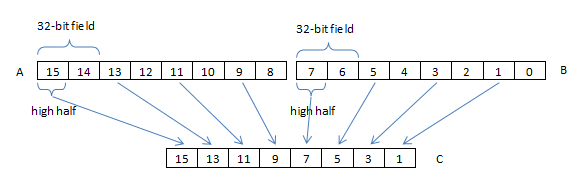
\includegraphics[width=130mm]{draw/packh_16.png}
\caption[Packh on 32-bit field width vectors.]{Packh operation. To be simple, packh on 32-bit field is shown here and the vectors are viewed as $v8i16$ and the indexes for the shuffle mask are drawn in the cell.}
\label{figure:packh_16}
\end{figure}

\begin{program}
\begin{verbatim}
  define <4 x i32> @packh_16(<4 x i32> %a, <4 x i32> %b) alwaysinline {
  entry:
    %aa = bitcast <4 x i32> %a to <16 x i8>
    %bb = bitcast <4 x i32> %b to <16 x i8>
    %rr = shufflevector <16 x i8> %bb, <16 x i8> %aa, <16 x i32> <i32 1, i32 3,
          i32 5, i32 7, i32 9, i32 11, i32 13, i32 15, i32 17, i32 19, i32 21,
          i32 23, i32 25, i32 27, i32 29, i32 31>

    %rr1 = bitcast <16 x i8> %rr to <4 x i32>
    ret <4 x i32> %rr1
  }
\end{verbatim}
\caption[Shufflevector implementation of packh.]{Shufflevector implementation of packh, it is machine independent. {\tt <4 x i32>} is a general vector type we use for all SIMD registers to simplify function interface.}
\label{program:packh_16}
\end{program}

In this program, we first bitcast operands into $i8$ vectors. "Bitcast" is also a useful LLVM operation that converts between integer, vector and FP-values; it changes the data type without moving or modifying the data; so it requires the source and result type to have the same bit size. We then fill in the indexes of all the high bits in order, which is 1, 3, \ldots, 31. Target-specific logic is thus left to the LLVM back end and is no longer the burden of the programmer. We optimize LLVM back end for better code generation later in this thesis.

For \verb|hsimd<16>::packl| which packs all the low bits of each 16-bit field, we just change the mask to be 0, 2, 4, 6, \ldots, 30; for {\tt packh} with different field width $w$, we can first bitcast the operands into vectors of $w/2$ element, and then shuffle with the similar increasing odd number mask. We also write the code of \verb|esimd<8>::mergeh| in Program~\ref{program:mergeh_8}, where the function is self-explanatory and any programmer who understands shufflevector can understand it easily.

\begin{program}
\begin{verbatim}
  define <4 x i32> @mergeh_8(<4 x i32> %a, <4 x i32> %b) alwaysinline {
  entry:
    %aa = bitcast <4 x i32> %a to <16 x i8>
    %bb = bitcast <4 x i32> %b to <16 x i8>
    %rr = shufflevector <16 x i8> %bb, <16 x i8> %aa, <16 x i32> <i32 8,
          i32 24, i32 9, i32 25, i32 10, i32 26, i32 11, i32 27, i32 12,
          i32 28, i32 13, i32 29, i32 14, i32 30, i32 15, i32 31>

    %rr1 = bitcast <16 x i8> %rr to <4 x i32>
    ret <4 x i32> %rr1
  }
\end{verbatim}
\caption[Shufflevector implementation of mergeh.]{Shufflevector implementation of mergeh, the function is self-explanatory and easy to understand.}
\label{program:mergeh_8}
\end{program}

However, the shufflevector has one limitation: the {\tt mask} can only contain constant integers, which prevents us from generating dynamic shuffle operation. Parabix deletion algorithm, for instance, takes two SIMD registers as input: A and DeletionMask. It will delete the bits from A at the locations marked by DeletionMask (delete the $i_{th}$ bit of A if $\text{DeletionMask}_i = 1$) and shift the rest of A to the lower end. This algorithm cannot be implemented in shufflevector because DeletionMask is not a constant. Given a DeletionMask, one can construct a shuffle mask to do both deletion and shifting, but LLVM does not support dynamic shuffle masks generated during the run time.

\section{Move SIMD Implementation Into The Back End}

This is our second principle and it is the nature complement of the first one. Instructions with accurate semantics like shufflevector are powerful, but may not be supported directly by the hardware yet. We move all the implementation knowledge we gained from the IDISA library into the LLVM back end and this implementation have to be mostly target-dependent for better performance. We will discuss in greater detail in Chapter~\ref{four} and Chapter~\ref{five} of how Parabix operations are lowered in our back end.

With these two principles, we get a big picture of the optimization framework like this: each function of the Parabix operation in IR are coded with sufficient semantics which would allow the compiler front end to optimize with enough context information while the back end would optimize on top of the SelectionDAG generated within the scope of a single function, the same scope with the IDISA generator.
